% Main file: connects the front matter, the chapters and the bibliography.
% Compile: bash scripts/build.sh  (output: build/main.pdf)
% Design: style/report.cls ("Creator's Pre-Production Journal").
\documentclass{style/report}

% IEEE-style bibliography (STY-07). Sources come only from docs/sources.md.
% NOTE: backend=bibtex because biber.exe hangs on this machine (even `biber --version`).
\usepackage[backend=bibtex,style=ieee]{biblatex}
\addbibresource{bib/references.bib}
% Keep titles exactly as written in the source, and use font-safe quote marks.
\DeclareFieldFormat{sentencecase}{#1}
\DeclareFieldFormat{titlecase}{#1}
\DeclareFieldFormat[article,inproceedings,online,misc,report,techreport,book,unpublished,inbook,incollection]{title}{{\fontspec{Times New Roman}\char"201C}#1{\fontspec{Times New Roman}\char"201D}}
% Allow long URLs/DOIs to break across lines (avoids overfull boxes in the reference list).
\setcounter{biburlnumpenalty}{100}
\setcounter{biburlucpenalty}{100}
\setcounter{biburllcpenalty}{100}

\begin{document}

% ---- Front matter (separate numbering) ----
\pagenumbering{roman}
% Title page: no page number (FRT-01). No ID numbers or emails (FRT-02).
\begin{titlepage}
  \thispagestyle{empty}
  \centering
  {\Large\bfseries אוניברסיטת חיפה \par}
  {\large המחלקה למדעי הנתונים \par}
  \vspace{1.8cm}
  {\Huge\bfseries דוח מכין \par}
  \vspace{1.4cm}
  {\LARGE פלטפורמת סוכני בינה מלאכותית לניהול רציפות עלילתית בסדרות וידאו עם דמויות קבועות, מתיאור מילולי בעברית \par}
  \vspace{1cm}
  \begin{english}
    {\large A Hebrew-First Multi-Agent ``Showrunner'' Platform for Narrative-Consistent AI Video Series \par}
  \end{english}
  \vspace{1.8cm}
  {\large שמות הסטודנטיות: יעלת חן פרידמן, עדי ניקול זכרוב \par}
  \vspace{0.3cm}
  {\large מנחה: ד״ר יורם סגל \par}
  \vspace{0.3cm}
  {\large שם הקורס: סוכני \textenglish{AI} ו־\textenglish{Vibe Coding} \par}
  \vfill
  {\large נובמבר 2026 \par}
\end{titlepage}

% Executive summary (250-350 words, written LAST) + keywords (5-7). FRT-03, FRT-04.
\chapter*{תקציר מנהלים}
\addcontentsline{toc}{chapter}{תקציר מנהלים}

% TODO: write last, one continuous paragraph: background, problem, solution, deliverables, milestones.

\section*{מילות מפתח}
% TODO: 5-7 technical keywords.

\tableofcontents
\listoffigures
\listoftables
% Abbreviations and terms, alphabetical, with full definitions (FRT-06).
\chapter*{רשימת קיצורים ומונחים}
\addcontentsline{toc}{chapter}{רשימת קיצורים ומונחים}

% TODO: fill in alphabetical order as terms appear in the report.


% ---- Body (pages 1-40) ----
\cleardoublepage
\pagenumbering{arabic}
% Page budget: 3 pages
\chapter{מבוא}

\section{מגמות בתחום}
שוק כלי יצירת הווידאו מבוססי בינה מלאכותית (\textenglish{AI}) גדל בקצב דו־ספרתי~\cite{fbi2026aivideo}, והיצירה האוטומטית של וידאו הופכת מניסוי טכנולוגי למוצר מסחרי [TO-VERIFY].לפי חברת הניתוח \textenglish{Fortune Business Insights}, היקף שוק מחוללי הווידאו מבוססי \textenglish{AI} הוערך ב־\textenglish{716.8} מיליון דולר ב־\textenglish{2025}, צפוי להגיע ל־\textenglish{847} מיליון דולר ב־\textenglish{2026}, ולצמוח ל־\textenglish{3,350} מיליון דולר ב־\textenglish{2034}, בקצב צמיחה שנתי מצטבר (\textenglish{CAGR}) של \textenglish{18.8}\% בתקופה \textenglish{2026--2034}~\cite{fbi2026aivideo}. צפון אמריקה החזיקה בכ־\textenglish{41}\% מהשוק ב־\textenglish{2025}~\cite{fbi2026aivideo}. נתון זה מעיד על ריכוז גיאוגרפי משמעותי של השוק ביבשת אחת.

הערכות השוק אינן אחידות. דוח ישן וצר יותר של \textenglish{Markets\-and\-Markets} הגדיר את שוק הטקסט־לווידאו (\textenglish{Text-to-Video}) כ־\textenglish{0.1} מיליארד דולר ב־\textenglish{2022} ו־\textenglish{0.9} מיליארד דולר ב־\textenglish{2027}, עם \textenglish{CAGR} של \textenglish{37.1}\%~\cite{mnm2023t2v}. ההפרש בין הדוחות נובע מהגדרות שונות של השוק, ולכן הדוח הנוכחי מתייחס לנתונים אלה כאל טווח ולא כאל מספר יחיד. פרק~4 מפרט את ההשוואה.

במקביל גדלה כלכלת היוצרים (\textenglish{Creator Economy}). לפי הערכת \textenglish{Goldman Sachs Research}, היקפה הפוטנציאלי עשוי לעלות מכ־\textenglish{250} מיליארד דולר ב־\textenglish{2023} לכ־\textenglish{480} מיליארד דולר ב־\textenglish{2027}~\cite{goldman2023creator}. אולם רק כ־\textenglish{4}\% מהיוצרים הם מקצועיים, כלומר מרוויחים יותר מ־\textenglish{100} אלף דולר בשנה~\cite{goldman2023creator}. הנתונים מרמזים על קהל לא מבוטל של יוצרים עצמאיים. קהל זה מחפש כלים שיאפשרו להם להפיק תוכן ברמה גבוהה בלי צוות הפקה.

\section{הקשר יישומי}
התחום היישומי של הדוח הוא סדרות וידאו קצרות סביב דמויות קבועות, המופצות ביוטיוב ובטיקטוק. בסדרה כזו הצופה חוזר לפרק הבא משום שהוא מכיר את הדמויות ואת העולם, ולכן הערך של הסדרה תלוי ברציפות. הרציפות כוללת שני רבדים: עקביות חזותית, כלומר הדמות נראית זהה משוט לשוט, ורציפות עלילתית, כלומר אירועי עבר, יחסים בין דמויות ומצבן נשמרים מפרק לפרק.

קהל היעד העיקרי הוא יוצרי תוכן דוברי עברית ללא רקע טכני. הרחבה עתידית אפשרית היא משרדי פרסום, שבהם דמויות מותג וקמפיינים מתמשכים דורשים את אותה רציפות. היקף קהל היעד בישראל הוא [TO-VERIFY] יוצרים.

כיום מי שמבקש להפיק סדרה כזו משתמש בכמה כלים נפרדים. קיימים כלים מסחריים כגון \textenglish{LTX Studio}~\cite{ltxstudio}, \textenglish{OpenArt}~\cite{openart} ו־\textenglish{LongStories.ai}~\cite{longstories}, וכן תהליך ידני המשלב כלי עריכה כמו \textenglish{CapCut}~\cite{capcut}. המוצרים האלה נבדקים לעומק בפרק~4.

\section{מוטיבציה}
הפתרונות הקיימים אינם מספקים יוצר שמבקש להפעיל סדרה ארוכה בעברית, מארבע סיבות. ראשית, התהליך מפוצל: היוצר מחבר בעצמו מודל תמונה, מודל וידאו, קול ועריכה, והמידע על הדמויות אינו נשמר במקום אחד. שנית, ניהול הרציפות העלילתית מוטל על היוצר. לפי בדיקת הצוות, הכלים שומרים על מראה הדמות ועל עולמה, ואחד מהם, \textenglish{LongStories.ai}, שומר גם על הדמויות, הקולות והעולם בין פרקים~\cite{longstories}, אך אינם מתעדים את אירועי העלילה ואינם מתריעים כשפרק חדש סותר פרק קודם [TO-VERIFY]. משמעות הדבר היא שהיוצר נדרש לזכור בעצמו מה אירע בכל פרק קודם ולבדוק ידנית שהפרק החדש אינו סותר אותו. שלישית, תמיכה בעברית בקלט, בקול, בסנכרון שפתיים ובכתוביות מימין לשמאל (\textenglish{RTL}) אינה מתועדת במקור: [TO-VERIFY]. רביעית, זמן ההפקה של דקת וידאו בתהליך הידני הוא [TO-VERIFY] שעות, ועלות הדקה היא [TO-VERIFY] דולר.

המחקר האקדמי מתמקד בעיקר בעקביות חזותית של דמויות ושל סצנות. עבודות כמו \textenglish{MovieDreamer}~\cite{zhao2025moviedreamer} ו־\textenglish{StoryDiffusion}~\cite{zhou2024storydiffusion} שומרות על זהות הדמות לאורך רצף ארוך, ו־\textenglish{StoryAgent}~\cite{hu2024storyagent} מציגה צוות סוכנים להפקה. סקירה מלאה מופיעה בפרק~3. הפער שמתגלה הוא שאף אחד מהם אינו מנהל זיכרון של העלילה עצמה ואינו מזהה סתירות עלילתיות בין פרקים, ואין מערכת קצה־לקצה הנגישה ליוצרים בעברית בלי תשלום.

\begin{directornote}
הפרויקט נולד מהפער הזה: מערכת של סוכנים בינה מלאכותית הפועלת כ״מנהל סדרה״ (\textenglish{Showrunner}), המנהלת ״ספר סדרה״ שמתעדכן אחרי כל פרק, מתריעה על סתירות ומקבלת קלט בעברית. הצלחת הפרויקט תימדד ביכולת לשמור על הדמות ועל העלילה לאורך פרקים, ולא רק בבניית עוד מחולל וידאו.
\end{directornote}

\section{מבנה הדוח}
הדוח בנוי כמשפך, מהרחב אל המסוים: הוא נפתח במגמות השוק, ממשיך להקשר היישומי ולמוטיבציה, וממשיך משם אל הבעיה, הספרות, השוק, התכן ותוכנית העבודה.פרק~2 מגדיר את הבעיה בצורה כמותית ומציג יעדי תכן ומפרט דרישות. פרק~3 סוקר את הספרות באופן תמטי, מנתח מאמר דגל ומנסח את פער הידע. פרק~4 מעריך את היקף השוק ומשווה בין מוצרים מתחרים. פרק~5 משווה חלופות תכן במטריצת החלטה משוקללת, ומציג את הארכיטקטורה המוצעת ואת החדשנות. פרק~6 מציג את תוכנית העבודה לסמסטר ב׳, הכוללת חלוקת משימות ולוח זמנים של ארבעה־עשר שבועות. פרק~7 מנתח סיכונים ופעולות מנע, ופרק~8 מסכם את הממצאים ואת שלוש הפעולות המיידיות לאחר אישור הדוח.

% Page budget: 4 pages
\chapter{הגדרת הבעיה}

\section{ניסוח הבעיה}
\subsection{מצב מצוי}
\subsection{מצב רצוי}

\section{יעדי תכן}

\section{מפרט דרישות}
\subsection{דרישות תפקודיות}
\subsection{דרישות לא־תפקודיות}

% Page budget: 9 pages
\chapter{סקירת ספרות}

\section{סקירה תמטית}
\subsection{עקביות חזותית של דמויות}
\subsection{רציפות עלילתית}
\subsection{יצירת וידאו מקצה לקצה}

\section{מטריצת ספרות}

\section{מאמר הדגל}
\subsection{בחירת המאמר}
\subsection{ניתוח המאמר}

\section{פער הידע}

% Page budget: 6 pages
\chapter{סקר שוק ומתחרים}

\section{היקף השוק}
היקף השוק מוצג בשלוש שכבות: שוק כולל (\textenglish{TAM}) שמבוסס על דוחות אנליסטים, ושוק זמין (\textenglish{SAM}) ושוק יעד (\textenglish{SOM}) שהם אומדני צוות שקופים ואינם נתוני מקור.

\subsection{שוק כולל}
שוק מחוללי הווידאו מבוסס הבינה המלאכותית נאמד ב־716.8 מיליון דולר ב־2025 וב־847 מיליון דולר ב־2026, עם תחזית של 3,350 מיליון דולר ב־2034 ושיעור צמיחה שנתי מורכב (\textenglish{CAGR}) של 18.8\% לתקופה 2026--2034 \cite{fbi2026aivideo}. נתח צפון אמריקה בשוק עמד על 41\% ב־2025 \cite{fbi2026aivideo}. דוח ישן וצר יותר, שמגדיר רק את שוק הטקסט־לווידאו, מעריך 0.9 מיליארד דולר ב־2027 (לעומת 0.1 מיליארד ב־2022) ושיעור צמיחה של 37.1\%, ללא תקופה מוצהרת בסיכום המקור\textenglish{[TO-VERIFY]} \cite{mnm2023t2v}.

שני המקורות מציגים אפוא טווח ולא מספר יחיד: סדר גודל של כ־0.85 עד 0.9 מיליארד דולר סביב 2026--2027, ושיעור צמיחה בין 18.8\% ל־37.1\%. הטווח אינו השוואה שווה, משום שהגדרות השוק שונות, תקופות התחזית שונות והדוח השני נכתב בפברואר 2023. לכן השוק הכולל משמש כאן להערכת סדר גודל בלבד.

\subsection{שוק זמין}
\textbf{אומדן צוות, לא נתון ממקור.} השוק הזמין הוא יוצרי תוכן דוברי עברית שמפעילים סדרות סביב דמויות קבועות. ההנחות: מספר היוצרים כאלה הוא כ־100,000 \textenglish{[TO-VERIFY]}, והם משלמים, לפי הנחת הצוות, מחיר חודשי של 25 דולר \textenglish{[TO-VERIFY]}, שהוא אמצע טווח יעד התכנון של 20 עד 30 דולר (לא נתון שנמדד). התוצאה היא 100,000 כפול 25 כפול 12, כלומר כ־30 מיליון דולר בשנה, שהם כ־3.5\% מהשוק הכולל של 2026. כל אחת משתי ההנחות דורשת אימות לפני ההגשה.

\subsection{שוק יעד}
\textbf{אומדן צוות, לא נתון ממקור.} השוק היעד הוא הנתח שניתן להשיג בשנה הראשונה לאחר השקה. ההנחה: חדירה של 0.5\% מהשוק הזמין \textenglish{[TO-VERIFY]}, כלומר כ־500 משתמשים משלמים. בעלות של 300 דולר למשתמש בשנה (25 דולר כפול 12 חודשים, \textenglish{[TO-VERIFY]}) התוצאה היא כ־150 אלף דולר בשנה. ההנחה זהירה בכוונה, כי היא נשענת על ערוץ הפצה אחד, קהילות יוצרים בעברית, ועל יכולת ייצור מוגבלת של צוות קטן.

\section{מתחרים}
הסקירה מתמקדת בארבעה כלי וידאו מבוססי בינה מלאכותית ובתהליך ידני אחד, ומעריכה כל אחד לפי יכולותיו המתועדות בדפי המוצר ולא לפי פרסומת.

\subsection{ניתוח טכני של מוצרים מתחרים}
חמישה מוצרים נסקרו, והמחירים הם מחירי מנוי חודשי בדולרים נכון ל־21.11.2026; מנוי שנתי זול יותר ואינו משמש כאן. \textenglish{LTX Studio} \cite{ltxstudio} מציע דמויות שמורות (\textenglish{Elements}) מהתוכנית הרגילה, ב־35 דולר, ושליטה גבוהה ביוצר באמצעות לוח תכנון (\textenglish{storyboard}) ובקרת מצלמה. \textenglish{OpenArt} \cite{openart} מציע דמויות עקביות כבר ב־14 דולר, אך תוכנית הבסיס אינה כוללת רישיון שימוש מסחרי. \textenglish{LongStories.ai} \cite{longstories} היא היחידה עם יכולת סדרה מפורשת: סרטון המשך הופך אוטומטית לפרק הראשון בסדרה, אך העלות הנדרשת היא 59 דולר בחודש. \textenglish{Atlabs} \cite{atlabs} מצהיר על תמיכה בעברית בתוכניות בתשלום בלבד, והדבר אושר בשיחה עם צוות התמיכה שלו.

\subsection{התהליך הידני כמתחרה}
תהליך ידני בעורך \textenglish{CapCut} \cite{capcut} הוא המתחרה הרביעי. ממשקו בעברית והוא זול, אך אינו יוצר וידאו, ולכן נדרשים כלי בינה מלאכותית נוספים וכל שלב נעשה ביד, כולל שמירת הרציפות בין הפרקים. המחיר המדווח הוא 19.99 דולר ל־\textenglish{Pro} \textenglish{[TO-VERIFY]}.

\section{טבלת השוואה}
טבלה~\ref{tab:ch4-compare} משווה את חמשת המוצרים, את מאמר הדגל \cite{zhao2025moviedreamer} ואת הפתרון המתוכנן לפי שישה פרמטרים, ונועדה להראות ששום מוצר אינו משלב בו־זמנית סדרה, עברית ויצירה מקצה לקצה. מאמר הדגל הוא מחקר ולא מוצר, ולכן אין לו מחיר, והוא מטפל בעלילה ובזהות דמות לאורך וידאו ארוך \cite{zhao2025moviedreamer}. עמודת הפתרון המתוכנן מציגה יעדי תכן ולא יכולות שנמדדו.

\begin{table}[h]
  \centering
  \caption{השוואה רב־פרמטרית: מוצרים, מאמר הדגל והפתרון המתוכנן (מחירים חודשיים בדולרים, 21.11.2026)}
  \label{tab:ch4-compare}
  \scriptsize
  \begin{tabular}{p{1.5cm} p{1.4cm} p{1.4cm} p{1.4cm} p{1.4cm} p{1.4cm} p{1.4cm} p{1.4cm}}
    \headrow \hcell{פרמטר} & \hcell{\textenglish{LTX Studio}} & \hcell{\textenglish{OpenArt}} & \hcell{\textenglish{Long\-Stories}} & \hcell{\textenglish{Atlabs}} & \hcell{\textenglish{CapCut} (ידני)} & \hcell{מאמר הדגל} & \hcell{פתרון מתוכנן} \\
    מנוי זול ביותר & 15 (\textenglish{Lite}) & 14 (\textenglish{Starter}) & 59 (\textenglish{Pro}) & 19 \textenglish{[TO-VERIFY]} & 19.99 \textenglish{[TO-VERIFY]} & אין, מחקר & יעד 20 עד 30 \\ \rowrule
    דמויות עקביות & כן, מ־35 & כן, מ־14 & כן & כן & לא & כן & כן \\ \rowrule
    סדרה ופרקים & לא נמצא & לא נמצא & כן & לא נמצא & לא & רצף ארוך, לא פרקים & כן, עם זיכרון עלילה \\ \rowrule
    עברית & לא נמצא & לא נמצא & לא נמצא & כן, בתשלום & כן, בממשק & לא נבדק & כן \\ \rowrule
    וידאו מקצה לקצה & כן & כן & כן & כן & לא & לא & כן \\ \rowrule
    חולשה עיקרית & אי אפשר לנסות בלי תשלום & טעינה ארוכה בלי תוצאה & אי אפשר לנסות בלי תשלום & עברית רק בתשלום & הכול ידני & אין מוצר זמין & טרם נבנה \\ \rowrule
  \end{tabular}
\end{table}

הטבלה מראה שהמוצרים התשלומיים מכסים עקביות ויצירה מקצה לקצה, אך רק אחד מכסה סדרה, ומבין ארבעת כלי הבינה המלאכותית רק אחד מצהיר על עברית. הערך ``לא נמצא'' פירושו שהנתון אינו מופיע בדפי המוצר הציבוריים או שלא ניתן היה לבדוק אותו בתוכנית חינמית; הוא אינו קביעה שהיכולת חסרה.

\section{ניתוח גרפי}
\subsection{תרשים רדאר}
איור~\ref{fig:ch4-radar} מציג פרופיל של שישה צירים בסולם 1 עד 5 לארבעה מתחרים ולפתרון המתוכנן, ונועד להראות שהפתרון המתוכנן שואף לכסות את הצירים שבהם המתחרים חלשים, בעיקר עברית ורציפות עלילתית. \textenglish{OpenArt} מופיע בטבלה בלבד. הציונים הם הערכת צוות: ציר העקביות גבוה בכל כלי בינה מלאכותית כי כולם מציעים דמויות שמורות; ציר העלות נקבע לפי מחיר הכניסה ליכולת העקביות; ציר העברית נמוך (1) כשלא נמצאה תמיכה; ורציפות עלילתית גבוהה רק ב־\textenglish{LongStories.ai}.

\begin{figure}[h]
  \centering
  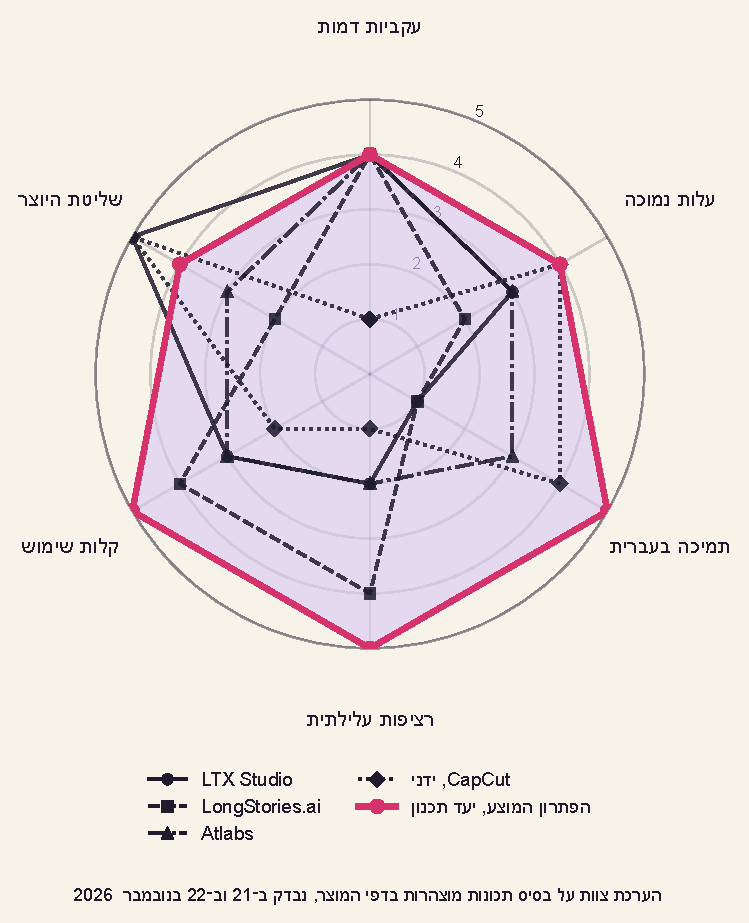
\includegraphics[width=0.8\textwidth]{figures/ch4_radar.pdf}
  \caption{תרשים רדאר: פרופיל ארבעה מתחרים ויעד התכנון. הערכת צוות על בסיס תכונות מוצהרות בדפי המוצר, נבדק ב־21.11.2026}
  \label{fig:ch4-radar}
\end{figure}

\subsection{גרף פיזור של יכולות מול עלות}
איור~\ref{fig:ch4-scatter} מעמת את מחיר התוכנית הזולה ביותר הכוללת דמויות עקביות עם מספר היכולות המרכזיות (מתוך ארבע) שבידי המוצר: דמויות עקביות, סדרה, עברית ווידאו מקצה לקצה. הגרף נועד להראות שאין מוצר בפינת הכיסוי המלא במחיר נמוך. נתוני עלות לדקת וידאו מוגמרת אינם זמינים, ולכן נבחרו ערכים שניתנים לאימות. יעד התכנון מסומן כיעד ולא כמוצר שנמדד.

\begin{figure}[h]
  \centering
  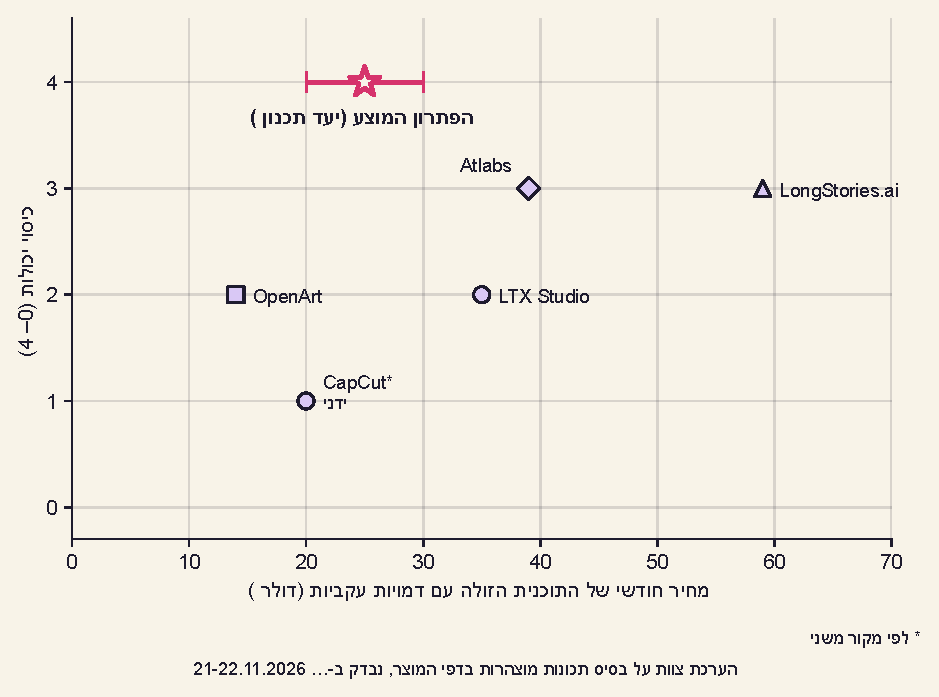
\includegraphics[width=0.8\textwidth]{figures/ch4_scatter.pdf}
  \caption{גרף פיזור: מחיר חודשי מול מספר יכולות מרכזיות. הערכת צוות על בסיס תכונות מוצהרות בדפי המוצר, נבדק ב־21.11.2026}
  \label{fig:ch4-scatter}
\end{figure}

\subsection{מגבלות הסקירה}
חלק מהכלים לא ניתנו לבדיקה ללא תשלום, ולכן ציוני קלות השימוש הם בחלקם הערכה. תמיכת \textenglish{Atlabs} בעברית מבוססת על התכתבות עם צוות התמיכה שלו ולא על בדיקה עצמאית. מחירי \textenglish{Atlabs} ו־\textenglish{CapCut} טרם אומתו מול דפי המחירים \textenglish{[TO-VERIFY]}, וכל הציונים בתרשים הרדאר הם שיפוט צוות. הסקירה אינה ממצה; קריטריוני בחירת חמשת המוצרים \textenglish{[TO-VERIFY]}, והנתונים הם תמונת מצב אחת מ־21.11.2026 שעשויה להשתנות.

\begin{directornote}
  בפרויקט שלנו הממצא המרכזי הוא שאף כלי לא נבדק בעברית בתוכנית חינמית, ולכן הפער הנגיש ליוצר דובר עברית נשאר פתוח. מחיר היעד של 20 עד 30 דולר נקבע כדי להימצא בטווח של המתחרים הזולים, ואומדני השוק הזמין והשוק היעד יעודכנו לאחר אימות ההנחות.
\end{directornote}

% Page budget: 8 pages
\chapter{חלופות תכן והחלטה}

הפרק בוחר בין שלוש גישות תכן שונות עקרונית באמצעות מטריצת החלטה משוקללת, ומראה שהחלופה ההיברידית מובילה בכל תרחישי בדיקת הרגישות. לאחר מכן הוא מציג את הארכיטקטורה ואת זרימת הנתונים של המערכת הנבחרת, ומסיים בהגדרה מנומקת של החדשנות. המשקלים והציונים בפרק הם הערכה של הצוות שאושרה על ידי חבריו, ואינם עובדות ממקור חיצוני. לכן הם מוצגים כהערכה בכל מקום שבו הם מופיעים, והדוח אינו מייחס להם תוקף של מדידה.

\section{חלופות תכן}
\label{sec:ch5-alternatives}
שלוש החלופות נבדלות בשאלה היסודית היכן נמצאת יכולת היצירה של הווידאו: בתוך הצוות, אצל ספק חיצוני, או בשילוב ביניהם. טבלה~\ref{tab:ch5-alternatives} מציגה לכל חלופה את היתרון העיקרי ואת המחיר שלו, והיא מראה שאין חלופה שאינה דורשת פשרה.

\begin{table}[h]
  \centering
  \caption{שלוש חלופות התכן: יתרון ומחיר}
  \label{tab:ch5-alternatives}
  \small
  \begin{tabular}{p{3.6cm} p{4.6cm} p{4.6cm}}
    \headrow \hcell{חלופה} & \hcell{יתרון} & \hcell{מחיר} \\
    \textbf{א׳:} מודל וידאו ייעודי שאומן או כוונן בידי הצוות & שליטה מלאה ועלות שולית נמוכה בהמשך & עלות פיתוח וחישוב גבוהה מאוד וזמן פיתוח ארוך \\ \rowrule
    \textbf{ב׳:} שכבת סוכנים מעל מודלים מסחריים דרך \textenglish{API} & זמן פיתוח קצר ואיכות גבוהה & תלות בספקים ועלות לדקה \\ \rowrule
    \textbf{ג׳:} היברידי: מודלים בקוד פתוח מקומית, ו־\textenglish{API} רק לשוטים קשים & איזון בין עלות לשליטה & מורכבות תפעולית, ונדרשת יחידת עיבוד גרפי (\textenglish{GPU}) \\
  \end{tabular}
\end{table}

חלופה א׳ מעניקה שליטה מלאה, אך היא דורשת אימון והערכה של מודל וידאו, ומשימה כזו אינה ניתנת להשלמה בסמסטר של ארבעה־עשר שבועות. חלופה ב׳ מקצרת את הפיתוח משום שהמודלים מוכנים, אך כל שנייה שנוצרת מחויבת, והמוצר חשוף לשינויי מחיר, ממשק ומדיניות של הספק. חלופה ג׳ מפצלת את העומס: מודלים בקוד פתוח מייצרים את רוב השוטים במקום, וקריאה לשירות חיצוני נשמרת לשוטים הקשים בלבד. המחיר הוא מורכבות תפעולית, כי נדרשים הקמת תשתית \textenglish{GPU} ולוגיקת ניתוב בין המודלים.

ההבדל בין שלוש החלופות הוא עקרוני ולא כמותי. בחלופה א׳ הצוות הוא בעל המודל, ולכן כל שיפור באיכות הוא עבודת מחקר שלו. בחלופה ב׳ המודל שייך לספק, והצוות מתמקד בתזמור ובזיכרון העלילה. בחלופה ג׳ הצוות בוחר לכל שוט את המקור המתאים ביותר, ולכן הוא מחזיק גם מודלים וגם חוזים עם ספקים. שלוש הגישות מובילות לפרופילים שונים של סיכון: חלופה א׳ מסתכנת בכך שהפרויקט לא יושלם, חלופה ב׳ בכך שמחיר או מדיניות של ספק יפגעו במוצר, וחלופה ג׳ בכך שהמורכבות התפעולית תחרוג מהיכולת של צוות קטן. הפרויקט עוסק בניהול רציפות עלילתית ולא באימון מודלי וידאו, ולכן חלופה א׳ מרחיקה את הצוות מהשאלה המרכזית שלו, בעוד שחלופות ב׳ ו־ג׳ מותירות את המאמץ בשכבת הסוכנים והזיכרון.

מבחינה טכנית, חלופה א׳ מחייבת איסוף נתוני וידאו, כוונון של מודל קיים וכתיבת תשתית הערכה, ובנוסף בניית קול וסנכרון שפתיים בעברית מאפס. הסיכון המרכזי הוא שהמאמץ ייבלע בהנדסת מודל בלי שיגיע לניהול הסדרה, ולכן הציון הנמוך בזמן הפיתוח ובאיכות, והציון הגבוה בתלות בספק ובפרטיות, נובעים כולם מאותה בחירה: הכול נשאר בבית.

חלופה ב׳ בנויה משכבת תזמור דקה מעל שירותי תמונה, וידאו וקול של ספקים. הסיכון המרכזי הוא חשיפה: שינוי מחיר, ממשק או מדיניות תוכן אצל ספק פוגע ישירות במוצר, ותמיכת העברית משתנה בין ספק לספק ואינה אחידה בין תמונה, קול וסנכרון שפתיים. לכן קיבלה חלופה זו את הציון הגבוה ביותר באיכות ובזמן הפיתוח, ואת הנמוך ביותר בתלות בספק.

חלופה ג׳ מוסיפה לשכבת התזמור רכיב ניתוב, מודלים פתוחים מקומיים וספק חיצוני כגיבוי. הסיכון המרכזי הוא עומס תפעולי על צוות קטן, ולכן זמן הפיתוח קיבל \textenglish{3} בלבד. האיכות גם היא נמוכה מזו של \textenglish{API} טהור, משום שרוב השוטים נוצרים במודלים פתוחים, אך העלות, העברית והפרטיות משתפרות, כי מודלי דיבור פתוחים בעברית נבחרים מקומית ורוב המידע אינו עוזב את המערכת.

\section{מטריצת החלטה}
\subsection{קריטריונים ומשקלים}
שישה קריטריונים נבחרו להשוואה, והמשקלים שלהם נקבעו לפני מתן הציונים, כדי שהציונים לא ישפיעו על חשיבות הקריטריונים. סכום המשקלים הוא \textenglish{1.0}. עקביות ואיכות קיבלה את המשקל הגבוה ביותר (\textenglish{0.25}) משום שהיא לב הבעיה שהפרויקט בא לפתור. עלות לדקה ותמיכה בעברית קיבלו \textenglish{0.20} כל אחד, כי הראשונה מגבילה את כדאיות ההפקה והשנייה היא מאפיין מגדיר של קהל היעד. זמן הפיתוח קיבל \textenglish{0.15} בשל מגבלת הסמסטר. תלות בספק ופרטיות ושליטה בקניין רוחני קיבלו \textenglish{0.10} כל אחד. המשקלים הם הערכה של הצוות ואושרו על ידו.

הסדר בין הקריטריונים משקף את מבנה הפרויקט. שני הקריטריונים הראשונים, עקביות ואיכות ועלות, יחד מהווים \textenglish{0.45} מהמשקל, משום שהם קובעים אם הסדרה ראויה לצפייה ואם אפשר להפיק אותה שוב ושוב. עברית נמדדת בנפרד ולא נכללת באיכות, כי חלופה יכולה להיות איכותית חזותית ועדיין לא לתמוך בקול ובכתוביות בעברית. שני הקריטריונים האחרונים קיבלו משקל נמוך יותר משום שהם משפיעים בעיקר על סיכון עתידי ולא על ההפקה בסמסטר הקרוב. כפי שמראה ניתוח הרגישות שלהלן, ההכרעה אינה תלויה בדיוק של משקלים אלה.

\subsection{ציונים וחישוב}
כל חלופה קיבלה ציון בין \textenglish{1} ל־\textenglish{5} בכל קריטריון, כשציון גבוה הוא תמיד טוב יותר: בעלות הציון \textenglish{5} פירושו הזול ביותר לדקה, ובתלות בספק \textenglish{5} פירושו התלות הנמוכה ביותר. הציון המשוקלל של חלופה $j$ מחושב לפי משוואה~\eqref{eq:ch5-score}:
\begin{equation}
  S_j = \sum_{i=1}^{6} w_i \, c_{ij}, \qquad \sum_{i=1}^{6} w_i = 1
  \label{eq:ch5-score}
\end{equation}
כאשר $w_i$ הוא משקל הקריטריון $i$, ו־$c_{ij}$ הוא ציון חלופה $j$ בקריטריון $i$. טבלה~\ref{tab:ch5-matrix} מציגה את המשקלים, את הציונים ואת הסכומים. הציונים הם הערכת צוות שאושרה על ידו ואינם נשענים על מקור, והנימוק לכל ציון מתועד בקובץ הנתונים של הפרויקט.

\begin{table}[h]
  \centering
  \caption{מטריצת החלטה משוקללת (משקלים וציונים: הערכת הצוות)}
  \label{tab:ch5-matrix}
  \small
  \begin{tabular}{p{4.6cm} c c c c}
    \headrow \hcell{קריטריון} & \hcell{משקל $w_i$} & \hcell{א׳} & \hcell{ב׳} & \hcell{ג׳} \\
    עקביות ואיכות & 0.25 & 2 & 4 & 3 \\ \rowrule
    עלות לדקה & 0.20 & 3 & 2 & 4 \\ \rowrule
    תמיכה בעברית & 0.20 & 3 & 3 & 4 \\ \rowrule
    זמן פיתוח & 0.15 & 1 & 5 & 3 \\ \rowrule
    תלות בספק & 0.10 & 5 & 1 & 3 \\ \rowrule
    פרטיות ושליטה בקניין רוחני & 0.10 & 5 & 2 & 4 \\ \rowrule
    \textbf{ציון משוקלל $S_j$} & \textbf{1.00} & \textbf{2.85} & \textbf{3.05} & \textbf{3.50} \\
  \end{tabular}
\end{table}

הנימוקים לציונים מבוססים על שיקול דעת של הצוות. בעקביות ואיכות קיבלה חלופה א׳ את הציון \textenglish{2}, משום שצוות קטן אינו צפוי להשיג בכוונון עצמי את האיכות החזותית של מודלי וידאו מובילים, וחלופה ב׳ קיבלה \textenglish{4} משום שמודלים מסחריים מספקים את האיכות הטובה ביותר הזמינה כיום. בעלות לדקה קיבלה חלופה ב׳ את הציון הנמוך \textenglish{2}, כי כל שנייה שנוצרת מחויבת. בזמן הפיתוח קיבלה חלופה א׳ את הציון \textenglish{1}, משום שאימון והערכה של מודל וידאו אינם משתלבים בסמסטר אחד. בתמיכה בעברית קיבלה חלופה ג׳ \textenglish{4}, כי אפשר לבחור מקומית מודלי דיבור פתוחים בעברית ולהשאיר ספק חיצוני כגיבוי. בתלות בספק ובפרטיות קיבלה חלופה ב׳ את הציונים הנמוכים, כי תסריטים ותמונות דמויות נשלחים לשירותי צד שלישי. מכיוון שהציונים אינם נשענים על מקור, הם נבחנים שוב בסמסטר ב׳ מול מדידות.

חלופה ג׳ מובילה עם \textenglish{3.50}, אחריה חלופה ב׳ עם \textenglish{3.05} וחלופה א׳ עם \textenglish{2.85}. איור~\ref{fig:ch5-decision} מפרק כל ציון לתרומות של הקריטריונים ($w_i c_{ij}$), ומאפשר לראות מהיכן נובע ההפרש. חלופה ב׳ מקבלת תרומה גבוהה מאיכות ומזמן פיתוח, אך תרומתה קטנה בעלות, בתלות בספק ובפרטיות. חלופה א׳ מקבלת תרומה גבוהה מתלות בספק ומפרטיות, אך כמעט אינה מקבלת תרומה מזמן פיתוח. חלופה ג׳ אינה הטובה ביותר בקריטריון בודד כלשהו מלבד עלות ועברית, אך היא היחידה שאינה מקבלת ציון נמוך מ־\textenglish{3} באף קריטריון, ולכן סכומה הגבוה ביותר.

\begin{figure}[h]
  \centering
  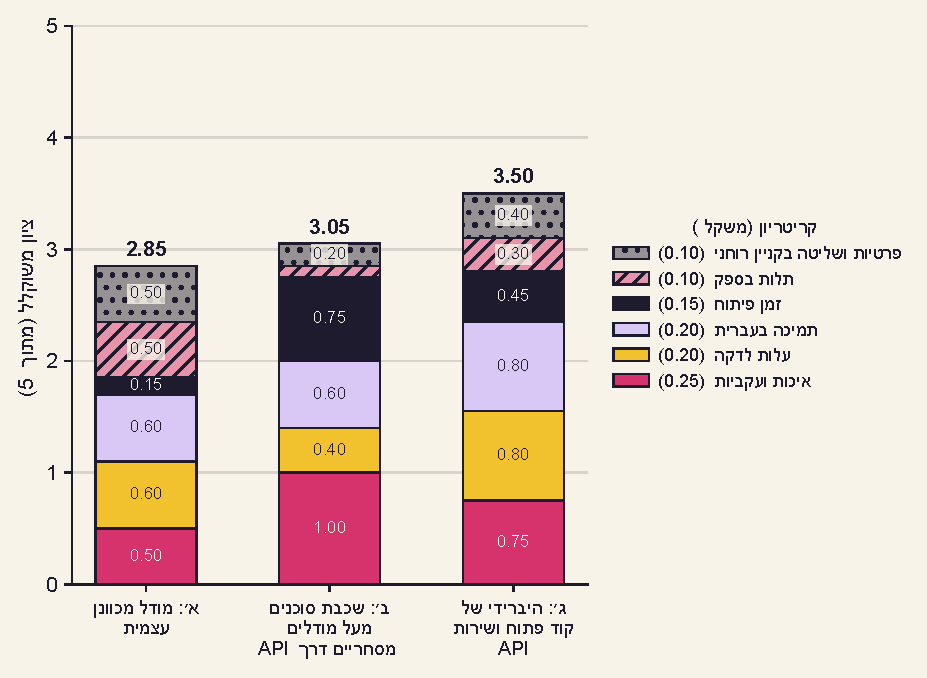
\includegraphics[width=0.8\textwidth]{figures/ch5_decision.pdf}
  \caption{תרומת כל קריטריון לציון המשוקלל של כל חלופה (משקלים וציונים: הערכת הצוות)}
  \label{fig:ch5-decision}
\end{figure}

\subsection{ניתוח רגישות}
בדיקת הרגישות בוחנת האם ההכרעה תלויה במשקלים שנבחרו. כל משקל הוזז בנפרד ב־\textenglish{0.1} כלפי מעלה וכלפי מטה, ושאר המשקלים הוקטנו או הוגדלו באופן יחסי כך שהסכום נשאר \textenglish{1.0}. בסך הכול נבדקו שנים־עשר תרחישים בנוסף למקרה הבסיס, והחישוב בוצע בקוד של הפרויקט. חלופה ג׳ ניצחה בכולם. ציונה נע בין \textenglish{3.43} ל־\textenglish{3.57}, והפער הקטן ביותר שלה מחלופה ב׳ נרשם כשמשקל זמן הפיתוח עלה ל־\textenglish{0.25}: \textenglish{3.44} מול \textenglish{3.28}, כלומר פער של \textenglish{0.16}. חלופה א׳ עקפה את חלופה ב׳ בארבעה תרחישים, אך לא את חלופה ג׳. בשני תרחישים משקל קריטריון אחד הופחת ל־\textenglish{0}, ובהם ג׳ עדיין ניצחה.

הפירוט מלמד על האופי של כל חלופה. חלופה ב׳ רגישה ביותר למשקל זמן הפיתוח: כשמשקלו יורד ל־\textenglish{0.05} ציונה יורד ל־\textenglish{2.82}, וכשהוא עולה ל־\textenglish{0.25} הציון עולה ל־\textenglish{3.28}. היא רגישה גם למשקלי האיכות והעלות: כשמשקל האיכות יורד ל־\textenglish{0.15} או כשמשקל העלות עולה ל־\textenglish{0.30}, ציונה יורד ל־\textenglish{2.92}. חלופה א׳ מרוויחה מהגדלת משקל התלות בספק ומשקל הפרטיות, ובכל אחד מהם היא מגיעה ל־\textenglish{3.09}, אך עדיין נשארת מאחורי חלופה ג׳ שמגיעה ל־\textenglish{3.44} ול־\textenglish{3.56} בהתאמה. חלופה ג׳ יציבה כי היא ממוצעת: אין לה ציון חריג כלפי מעלה או מטה, ולכן שינוי במשקל אחד אינו מזיז אותה בצורה חדה.

חשוב להדגיש את גבול המסקנה. הבדיקה מראה שההכרעה יציבה ביחס לשינוי המשקלים, אך אינה בודקת שינוי של הציונים עצמם, והציונים הם הערכה. שינוי בציון אחד, למשל ירידה באיכות של מודלים בקוד פתוח, עלול לצמצם את הפער, והדבר יידרש בדיקה חוזרת בסמסטר ב׳ לאחר מדידה בפועל.

\begin{directornote}
המטריצה לא נועדה להוכיח שחלופה ג׳ ״נכונה״, אלא לחשוף על אילו הנחות היא נשענת. ההנחה הרגישה ביותר היא הציון ״ג׳ בעקביות ואיכות: 3״. לכן המדידה הראשונה בסמסטר ב׳ תהיה השוואת איכות של שוט מקומי מול שוט דרך \textenglish{API}.
\end{directornote}

\section{הארכיטקטורה הנבחרת}
\subsection{ארכיטקטורת המערכת}
הארכיטקטורה היא צוות של שישה סוכנים הפועלים במעגל סביב זיכרון משותף, והיא מיישמת את חלופה ג׳ בשכבת התזמור. איור~\ref{fig:ch5-architecture} מציג את הסדר: שומר ספר הסדרה מספק את מצב העולם, כותב העלילה מציע את הפרק, והבמאי מתרגם אותו לסטוריבורד ולשוטים. מתזמר הייצור מפעיל את המודלים ומחליט איזה שוט יוצר מקומית ואיזה דרך \textenglish{API}, בדיוק כפי שחלופה ג׳ מגדירה. בודק הרציפות משווה את התוצר לספר הסדרה ומתריע על סתירות, ומנתח הקהל מזין את הצעות הפרק הבא. התוצאה חוזרת לשומר ספר הסדרה, וכך המעגל נסגר.

\begin{figure}[h]
  \centering
  \begin{tikzpicture}[
      box/.style={draw, rounded corners=3pt, minimum width=3.8cm, minimum height=1.7cm, align=center, text width=3.6cm, inner sep=3pt, font=\small},
      keep/.style={box, very thick, fill=black!8},
      arr/.style={->, thick}]
    \node[keep] (a) at (5,1.6) {\textbf{1. שומר ספר הסדרה}\\ זיכרון עולם ועלילה};
    \node[box]  (b) at (0,1.6) {\textbf{2. כותב העלילה}\\ הצעת פרק};
    \node[box]  (c) at (-5,1.6) {\textbf{3. במאי}\\ סטוריבורד ושוטים};
    \node[box]  (d) at (-5,-1.6) {\textbf{4. מתזמר הייצור}\\ ניתוב בין מודלים};
    \node[box]  (e) at (0,-1.6) {\textbf{5. בודק רציפות}\\ זיהוי סתירות};
    \node[box]  (f) at (5,-1.6) {\textbf{6. מנתח קהל}\\ תגובות וצפיות};
    \draw[arr] (a) -- (b);
    \draw[arr] (b) -- (c);
    \draw[arr] (c) -- (d);
    \draw[arr] (d) -- (e);
    \draw[arr] (e) -- (f);
    \draw[arr] (f) -- (a);
  \end{tikzpicture}
  \caption{ארכיטקטורת צוות הסוכנים: מעגל סגור סביב ספר הסדרה}
  \label{fig:ch5-architecture}
\end{figure}

תפקידי הסוכנים מוגדרים לפי הקלט והפלט של כל אחד. שומר ספר הסדרה מקבל פרק מוגמר ומחלץ ממנו אירועים, יחסים ושינויים במצב הדמויות, וכותב אותם לספר. כותב העלילה קורא את הספר ואת בקשת המשתמש ומפיק תסריט לפרק הבא. הבמאי מפרק את התסריט לסצנות, לסטוריבורד ולשוטים, ומציין לכל שוט אילו דמויות מופיעות בו. מתזמר הייצור מקבל רשימת שוטים ומפעיל מודלי תמונה, וידאו וקול. בודק הרציפות מקבל את הפרק ואת הספר, ומחזיר רשימת סתירות אפשריות עם הנימוק לכל אחת. מנתח הקהל מקבל נתוני צפייה ותגובות אחרי הפרסום ומחזיר הצעות להמשך. חלוקה כזו מאפשרת לבדוק כל סוכן בנפרד, ולהחליף את המודל שמאחוריו מבלי לשנות את שאר המעגל, וזו התכונה שמצדיקה את בחירת חלופה ג׳ שבה הספקים ניתנים להחלפה.

הזרימה בין הסוכנים מועברת במבנים מוגדרים ולא בטקסט חופשי. בין שומר ספר הסדרה לכותב העלילה עובר מצב עולם: דמויות, אירועים ויחסים. בין כותב העלילה לבמאי עובר תסריט, ובין הבמאי למתזמר רשימת שוטים שלכל אחד מהם תיאור חזותי ורשימת דמויות. המתזמר מעביר לבודק הרציפות את הפרק שנוצר, והבודק מחזיר לבמאי או למתזמר דרישת תיקון כשנמצאה סתירה. מנתח הקהל מעביר לכותב העלילה הצעות מבוססות תגובות. בנוסף, ההפרדה מאפשרת לתעד כל מעבר, ולכן אפשר לדעת איזה סוכן גרם לשגיאה.

הארכיטקטורה קרובה לצוות ההפקה של \textenglish{StoryAgent} \cite{hu2024storyagent}, וכן לתפקיד הבמאי שמוצע במאמר \textenglish{VideoDirectorGPT} \cite{lin2023videodirectorgpt}. ההבדל הוא בשני הסוכנים שאינם מופיעים בהם כמטרה: שומר ספר הסדרה, שמחזיק מצב עלילה בין פרקים, ובודק הרציפות, שמשווה את הפרק החדש למצב הזה.

\subsection{תרשים זרימת נתונים}
תרשים זרימת הנתונים מראה מה עובר בין הרכיבים מרגע הקלט ועד הפרק המוגמר, ואיפה ספר הסדרה משמש כזיכרון משותף. כפי שמוצג באיור~\ref{fig:ch5-dataflow}, הקלט הוא טקסט או דיבור בעברית, והוא מומר לטקסט ומובן בשלב הראשון. שלבי הכתיבה והבימוי קוראים את ספר הסדרה כדי להישאר נאמנים לעולם, בודק הרציפות קורא אותו כדי לאתר סתירות, וספר הסדרה מתעדכן בסוף עם הפרק שנוצר. השלב של כתוביות ושמע בעברית נעשה לפני הפלט, כדי שהכתוביות יוצגו מימין לשמאל.

\begin{figure}[h]
  \centering
  \begin{tikzpicture}[
      box/.style={draw, rounded corners=3pt, minimum width=3.1cm, minimum height=1.5cm, align=center, text width=2.9cm, inner sep=3pt, font=\small},
      mem/.style={draw, very thick, rounded corners=3pt, fill=black!8, minimum width=7.4cm, minimum height=1.6cm, align=center, text width=7cm, font=\small},
      arr/.style={->, thick},
      link/.style={<->, dashed, thick}]
    \node[box] (in)  at (5.4,2.8)  {\textbf{קלט משתמש}\\ טקסט או דיבור בעברית};
    \node[box] (und) at (1.8,2.8)  {\textbf{הבנת הקלט}\\ תמלול וחילוץ כוונה};
    \node[box] (plot) at (-1.8,2.8) {\textbf{כתיבת עלילה}\\ תסריט הפרק};
    \node[box] (dir) at (-5.4,2.8) {\textbf{בימוי}\\ סטוריבורד ושוטים};
    \node[box] (prod) at (-5.4,-2.8) {\textbf{הפקה}\\ תמונה, וידאו וקול};
    \node[box] (chk) at (-1.8,-2.8) {\textbf{בדיקת רציפות}\\ סתירות מול הספר};
    \node[box] (asm) at (1.8,-2.8) {\textbf{הרכבה}\\ סנכרון שפתיים וכתוביות};
    \node[box] (out) at (5.4,-2.8) {\textbf{פרק מוגמר}\\ וידאו לפרסום};
    \node[mem] (bible) at (0,0) {\textbf{ספר הסדרה} (זיכרון משותף)\\ דמויות, אירועים, יחסים ומצב העולם};
    \draw[arr] (in) -- (und);
    \draw[arr] (und) -- (plot);
    \draw[arr] (plot) -- (dir);
    \draw[arr] (dir) -- (prod);
    \draw[arr] (prod) -- (chk);
    \draw[arr] (chk) -- (asm);
    \draw[arr] (asm) -- (out);
    \draw[link] (plot) -- (plot |- bible.north);
    \draw[link] (dir) -- (dir |- bible.north);
    \draw[link] (chk) -- (chk |- bible.south);
    \draw[arr, dashed] (out) -- (out |- bible.east) -- (bible.east);
  \end{tikzpicture}
  \caption{תרשים זרימת נתונים: מקלט בעברית לפרק מוגמר, וספר הסדרה כזיכרון משותף}
  \label{fig:ch5-dataflow}
\end{figure}

שלב ההפקה הוא המקום שבו חלופה ג׳ באה לידי ביטוי בזרימה. לכל שוט מוגדר מסלול: ברירת המחדל היא מודל בקוד פתוח שרץ על \textenglish{GPU} מקומי, ורק שוט שנכשל בבדיקת האיכות, או שדורש יכולת שהמודל המקומי אינו מספק, נשלח לספק דרך \textenglish{API}. ההנחה בבסיס הציונים בעלות ובפרטיות בטבלה~\ref{tab:ch5-matrix} היא שרק חלק מהשוטים יצא מהמערכת. שיעור השוטים הקשים אינו ידוע כעת, והוא יימדד בסמסטר ב׳.

התרשים מבהיר הבדל מעקרוני בין הארכיטקטורה לבין שרשרת כלים רגילה. בשרשרת רגילה המידע זורם בכיוון אחד ונעלם בסיומו, ואילו כאן הפרק המוגמר מעדכן את ספר הסדרה, והפרק הבא נכתב מתוך המצב המעודכן. החץ המקווקו מהפרק המוגמר אל ספר הסדרה הוא החיבור שמאפשר רציפות בין פרקים. בודק הרציפות ממוקם אחרי ההפקה וגם לפני ההרכבה, כדי שסתירה תתגלה לפני שהתוצר עובר שלבים יקרים נוספים.

\section{החדשנות}
\label{sec:ch5-innovation}
החדשנות של הפרויקט היא שילוב של זיכרון עלילה, זיהוי סתירות ועברית במערכת אחת, ולא רכיב טכנולוגי חדש. הטענה מבוססת על פער הידע שנוסח בפרק~3 (סעיף~\ref{sec:ch3-gap}): המחקרים והמוצרים הקיימים שומרים על עקביות חזותית של דמויות ועולם, ולעיתים גם בין פרקים, אך אף אחד מהם אינו מנהל זיכרון של העלילה עצמה ואינו מזהה סתירות עלילתיות, ואף אחד אינו נגיש כמערכת קצה־לקצה ליוצרים בעברית.

הניסוח זהיר במכוון. \textenglish{LongStories.ai} שומר על צוות דמויות, על קולות ועל עולם בין פרקים \cite{longstories}, ולכן אין בדוח טענה שדמויות קבועות בין פרקים הן חידוש. מוצרים נוספים בתחום, ובהם \textenglish{LTX Studio} \cite{ltxstudio}, נבחנים בפרק~4 כמתחרים, וההשוואה ביניהם לבין הפרויקט נשענת על נתוני השוק שם. מבין המאמרים, \textenglish{MovieDreamer} משלב תכנון ורינדור לשמירה על קוהרנטיות נרטיבית \cite{zhao2025moviedreamer}, ו־\textenglish{StoryAgent} מארגן סוכנים סביב סיפור יחיד \cite{hu2024storyagent}, אך לפי מטריצת הספרות בפרק~3 אף אחד מהם אינו מכסה זיכרון עלילה או עברית.

התרומה מורכבת משלושה רכיבים. הראשון הוא ״מנהל סדרה״: ספר סדרה שמתעדכן אחרי כל פרק, מציע המשך עלילה ומתריע על סתירות מול פרקים קודמים. השני הוא עברית קודם כול: קלט בדיבור או בטקסט בעברית, קול בעברית, סנכרון שפתיים וכתוביות מימין לשמאל לאורך כל התהליך. השלישי הוא סגירת מעגל עם הקהל, שבה ניתוח תגובות וצפיות מזין הצעות לפרק הבא. אף אחד מהרכיבים אינו מובטח לבדו כחדש, כי כל מוצר או מאמר מכסה חלק מהם, והטענה היא ששילובם בסדרה אחת, ובפרט השילוב של זיכרון עלילה עם עברית, לא נמצא במקורות שנבדקו. טענה כזו מוגבלת לרשימת המקורות הסגורה, והיא אינה סקירה מלאה של השוק.

הבחירה בחלופה ג׳ מחזקת את הטענה: מכיוון שהמודלים ניתנים להחלפה והמאמץ מתמקד בשכבת הסוכנים והזיכרון, ההשקעה של הצוות מופנית לפער שזוהה ולא לשיפור מודלי וידאו שאחרים כבר מפתחים. כך החדשנות נמדדת ביכולת המערכת לשמור על עלילה עקבית לאורך פרקים, ולא באיכות הפיקסלים של שוט בודד.

מכאן נגזר גם מבחן ההצלחה של התרומה: היכולת לזהות סתירות עלילתיות שנשתלו בכוונה בפרקים (ראו דרישה \textenglish{REQ-NAR-01}). אם הבודק אינו מגיע לסף שייקבע, החדשנות לא הוכחה, והפרויקט נשאר שרשרת כלים מסודרת בלבד.

% Page budget: 4 pages
\chapter{תוכנית עבודה}

\section{מבנה פירוק העבודה}
העבודה בסמסטר ב' מחולקת לחמש חבילות עבודה, שלכל אחת מהן תת־משימות ותוצר מוגדר. מבנה פירוק עבודה (\mbox{\textenglish{Work Breakdown Structure, WBS}}) מאפשר לקשור כל משימה לדרישה מפרק~2 ולבדוק אם התוצר הושג. איור~\ref{fig:ch6-wbs} מציג את המבנה ההיררכי, וטבלה~\ref{tab:ch6-wbs} מפרטת את תת־המשימות והתוצרים של כל חבילה.

\begin{figure}[h]
  \centering
  \resizebox{\textwidth}{!}{% WBS diagram: root + 5 work packages (right-to-left order, WP1 on the right).
\begin{tikzpicture}[
    root/.style={draw, very thick, rounded corners=3pt, fill=brandHighlight, minimum width=6.4cm, minimum height=0.9cm, align=center, font=\small\bfseries},
    wp/.style={draw, rounded corners=3pt, fill=paper, minimum width=2.45cm, text width=2.3cm, minimum height=2.1cm, align=center, inner sep=3pt, font=\footnotesize},
    outb/.style={draw, dashed, rounded corners=2pt, minimum width=2.45cm, text width=2.3cm, minimum height=0.9cm, align=center, inner sep=2pt, font=\scriptsize},
    ln/.style={thick, brandMain}]
  \node[root] (r) at (0,3.2) {פלטפורמת מנהל סדרה בעברית};
  \foreach \i/\x/\t/\o in {
      1/5.2/{\textbf{חבילה 1}\\ספר הסדרה ומודל הנתונים}/{ספר סדרה פעיל},
      2/2.6/{\textbf{חבילה 2}\\צוות הסוכנים והתזמור}/{צינור סוכנים},
      3/0/{\textbf{חבילה 3}\\שילוב מודלי תמונה, וידאו וקול}/{שוט עם קול וכתוביות},
      4/-2.6/{\textbf{חבילה 4}\\ממשק משתמש ומבחני שמישות}/{ממשק ודוח שמישות},
      5/-5.2/{\textbf{חבילה 5}\\בדיקות, תיעוד והגנה}/{דוח בדיקות ומצגת}} {
    \node[wp] (w\i) at (\x,0.7) {\t};
    \node[outb] (o\i) at (\x,-1.1) {\o};
    \draw[ln] (r.south) -- ++(0,-0.35) -| (w\i.north);
    \draw[ln, ->] (w\i.south) -- (o\i.north);
  }
\end{tikzpicture}
}
  \caption{מבנה פירוק עבודה: חמש חבילות עבודה}
  \label{fig:ch6-wbs}
\end{figure}

האיור מראה שהפרויקט מתפרק לחמש חבילות בלבד, כך שכל תת־משימה שייכת לחבילה אחת ואין משימה ללא תוצר. הסדר בטבלה הוא סדר הבנייה: תחילה הנתונים, אחריהם הסוכנים והמודלים, ולבסוף הממשק והבדיקות. כל תוצר נבדק מול הדרישה המתאימה מפרק~2 לפני שהחבילה הבאה נשענת עליו.

\begin{table}[h]
  \centering
  \caption{חבילות עבודה, תת־משימות ותוצרים}
  \label{tab:ch6-wbs}
  \begin{tabular}{p{2.9cm} p{5.6cm} p{3.4cm}}
    \headrow \hcell{חבילה} & \hcell{תת־משימות} & \hcell{תוצר} \\
    1. ספר הסדרה ומודל הנתונים & תכנון מבנה הנתונים של דמויות ועולם; שמירה ועדכון אחרי כל פרק & ספר סדרה פעיל \\ \rowrule
    2. צוות הסוכנים והתזמור & הגדרת תפקידי הסוכנים; חיבור ביניהם; בודק רציפות & צינור סוכנים מקצה לקצה \\ \rowrule
    3. שילוב מודלי תמונה, וידאו וקול & חיבור ספקים דרך ממשק תכנות; קול עברי; כתוביות מימין לשמאל & יצירת שוט עם קול וכתוביות \\ \rowrule
    4. ממשק משתמש ומבחני שמישות & בניית ממשק לקלט בעברית; מבחן עם משתמשים ללא רקע טכני & ממשק ודוח שמישות \\ \rowrule
    5. בדיקות, תיעוד והגנה & בדיקות מול הדרישות; תיעוד; הכנת ההגנה & דוח בדיקות ומצגת \\
  \end{tabular}
\end{table}

כל חבילה מקושרת לדרישה אחת לפחות מפרק~2. בחבילה~1 נבנה מבנה הנתונים של הדמויות והעולם, והתוצר, ספר סדרה פעיל, הוא הבסיס לבדיקת \textenglish{REQ-NAR-01}, משום שרק מצב שמור מאפשר להשוות פרק חדש לפרקים קודמים. בחבילה~2 מוגדרים תפקידי הסוכנים ובודק הרציפות, והתוצר הוא צינור מקצה לקצה; חבילה זו מאמתת את \textenglish{REQ-NAR-01} בפרקי בדיקה עם סתירות שתולות. בחבילה~3 מחוברים ספקי תמונה, וידאו וקול, והיא מאמתת את \textenglish{REQ-CHR-01} בהשוואת פנים בין סצנות, את \textenglish{REQ-LNG-01} בקול ובכתוביות בעברית ואת \textenglish{REQ-CST-01} בחישוב עלות לפי מחירוני ספקים. בחבילה~4 נבנה ממשק הקלט בעברית, ומבחן השמישות עם משתמשים ללא רקע טכני מאמת את \textenglish{REQ-UX-01}. בחבילה~5 מורצות כל הבדיקות, כולל סריקת הקוד של \textenglish{REQ-SEC-01}, ונכתבים התיעוד ומצגת ההגנה.

\section{חלוקת אחריות}
כל משימה מקבלת אחראית ביצוע אחת בלבד, והמנחה מאשר את התוצר. טבלה~\ref{tab:ch6-raci} מציגה את מטריצת האחריות (\textenglish{RACI}), שבה \textenglish{R} מבצעת, \textenglish{A} אחראית סופית, \textenglish{C} מתייעצת ואילו \textenglish{I} מעודכנת. הטבלה מראה שבכל שורה יש \textenglish{R} אחת וגם \textenglish{A} אחת, ושהמנחה הוא \textenglish{A} בכל החבילות. חלוקת התפקידים בין שתי הסטודנטיות היא הצעה ראשונית, והיא תיקבע סופית בתחילת הסמסטר.

\begin{table}[h]
  \centering
  \caption{מטריצת אחריות לפי חבילות עבודה}
  \label{tab:ch6-raci}
  \begin{tabular}{p{5.2cm} p{2.2cm} p{2.2cm} p{2.2cm}}
    \headrow \hcell{חבילה} & \hcell{סטודנטית א׳} & \hcell{סטודנטית ב׳} & \hcell{מנחה} \\
    1. ספר הסדרה ומודל הנתונים & \textenglish{R} & \textenglish{C} & \textenglish{A} \\ \rowrule
    2. צוות הסוכנים והתזמור & \textenglish{R} & \textenglish{C} & \textenglish{A} \\ \rowrule
    3. שילוב מודלי תמונה, וידאו וקול & \textenglish{C} & \textenglish{R} & \textenglish{A} \\ \rowrule
    4. ממשק משתמש ומבחני שמישות & \textenglish{C} & \textenglish{R} & \textenglish{A} \\ \rowrule
    5. בדיקות, תיעוד והגנה & \textenglish{R} & \textenglish{C} & \textenglish{A} \\
  \end{tabular}
\end{table}

\section{לוח זמנים ונתיב קריטי}
לוח הזמנים משתרע על ארבעה עשר שבועות, וקובע שתי אבני דרך, כל אחת עם שבוע רזרבה שקודם לה. תרשים גאנט (\mbox{\textenglish{Gantt chart}}) באיור~\ref{fig:ch6-gantt} מציג את משך כל חבילה, את התלויות ביניהן ואת הנתיב הקריטי, והוא נועד להראות אילו חבילות אינן יכולות להתעכב בלי לדחות את ההגשה.

\begin{figure}[h]
  \centering
  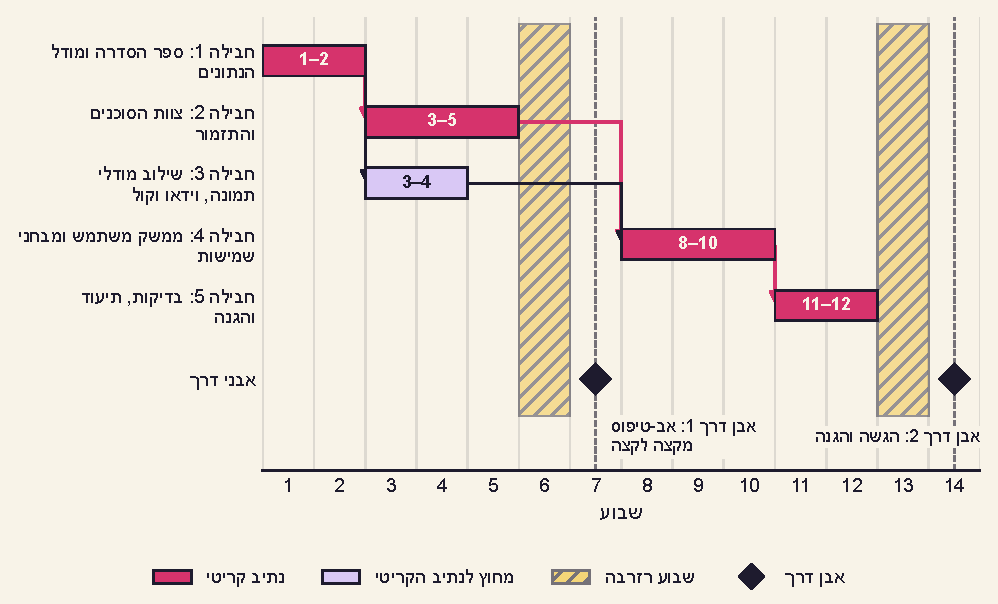
\includegraphics[width=\textwidth]{figures/ch6_gantt.pdf}
  \caption{תרשים גאנט: ארבעה עשר שבועות, נתיב קריטי ושתי אבני דרך}
  \label{fig:ch6-gantt}
\end{figure}

טבלה~\ref{tab:ch6-schedule} מסכמת את אותם נתונים במספרים: שבועות ההתחלה והסיום של כל חבילה, התלות שלה ומעמדה בנתיב הקריטי. היא מאפשרת לבדוק במבט אחד שכל חבילה מתחילה רק אחרי שהחבילות שהיא תלויה בהן הסתיימו.

\begin{table}[h]
  \centering
  \caption{לוח זמנים לפי חבילות עבודה (הערכת צוות)}
  \label{tab:ch6-schedule}
  \begin{tabular}{p{3.6cm} p{2.1cm} p{2.6cm} p{2.6cm}}
    \headrow \hcell{חבילה} & \hcell{שבועות} & \hcell{תלות} & \hcell{נתיב קריטי} \\
    1. ספר הסדרה ומודל הנתונים & \textenglish{1–2} & אין & כן \\ \rowrule
    2. צוות הסוכנים והתזמור & \textenglish{3–5} & חבילה 1 & כן \\ \rowrule
    3. שילוב מודלי תמונה, וידאו וקול & \textenglish{3–4} & חבילה 1 & לא \\ \rowrule
    4. ממשק משתמש ומבחני שמישות & \textenglish{8–10} & חבילות 2 ו־3 & כן \\ \rowrule
    5. בדיקות, תיעוד והגנה & \textenglish{11–12} & חבילה 4 & כן \\
  \end{tabular}
\end{table}

הנתיב הקריטי עובר דרך חבילה~1, חבילה~2, חבילה~4 וחבילה~5. חבילה~1 נמשכת בשבועות 1 עד 2, וחבילה~2 בשבועות 3 עד 5. אבן הדרך הראשונה בשבוע 7 היא אב־טיפוס מקצה לקצה, ושבוע 6 משמש לה רזרבה. חבילה~3 רצה במקביל לחבילה~2 בשבועות 3 עד 4, ואינה על הנתיב הקריטי, ולכן יש לה שבוע גמישות אחד. חבילה~4 נמשכת בשבועות 8 עד 10, וחבילה~5 בשבועות 11 עד 12. אבן הדרך השנייה בשבוע 14 היא הגשה והגנה, ושבוע 13 משמש לה רזרבה. משכי החבילות, התלויות ושבועות הרזרבה הם הערכת הצוות ולא נתון ממקור חיצוני, והם יעודכנו לאחר מדידת הקצב בפועל; מספר שעות העבודה השבועיות הזמינות הוא 20, כלומר שני סטודנטים כפול 10 שעות בשבוע (הנחת צוות).

לוגיקת התלויות פשוטה: חבילה אינה מתחילה לפני שהתוצר שהיא נשענת עליו מוכן. צוות הסוכנים תלוי בספר הסדרה משום שהסוכנים קוראים ממנו ומעדכנים אותו, והממשק תלוי באב־טיפוס הראשון משום שאין מה להציג לפני שהצינור פועל. חבילה~3 תלויה רק בספר הסדרה של חבילה~1, ולכן אפשר לבצע אותה במקביל לחבילה~2. הנתיב הקריטי הוא הרצף הארוך ביותר של חבילות תלויות, ולכן כל עיכוב בו מזיז ישירות את מועד ההגשה, בעוד עיכוב בחבילה~3 נספג בשבוע הגמישות שלה.

\begin{directornote}
  בפרויקט שלנו תלויות החבילות משקפות את הרעיון המרכזי: ספר הסדרה חייב להיות מוכן לפני צוות הסוכנים, ולכן עיכוב בחבילה~1 דוחה את כל הנתיב. הרזרבה בשבוע 6 נועדה לספוג בעיקר עיכוב כזה, ומבחן השמישות בחבילה~4 ייערך עם שמונה משתמשים חדשים (יעד תכנון).
\end{directornote}

\section{אבני דרך ובקרה}
בסוף כל אבן דרך נערכת בדיקה מול דרישות פרק~2. באבן הדרך הראשונה נבדקות עקביות הזהות ותפקוד הצינור מקצה לקצה, ובאבן הדרך השנייה נבדקות כלל הדרישות, כולל שמישות ועלות. אם חבילה על הנתיב הקריטי מתעכבת, שבוע הרזרבה שלפני אבן הדרך נצרך תחילה, ורק אחר כך מצומצם היקף של חבילה שאינה קריטית. כך נשמרת הגשה במועד בלי לוותר על התוצרים שהדרישות תלויות בהם. מדיניות הרזרבה קובעת שהשבוע אינו מתוכנן למשימות חדשות; הוא מנוצל רק לאחר עיכוב בפועל, ושבוע שלא נוצל משמש לתיקון ליקויים שנמצאו בבדיקה. בכל אבן דרך נערכת פגישת סקירה עם המנחה, שבה מוצג התוצר, מסומן סטטוס כל דרישה (עברה, נכשלה או טרם נבדקה) ומוחלט אם להמשיך בתוכנית או לצמצם היקף. סטייה של יותר משבוע אחד מהתכנון מדווחת למנחה באותו שבוע, וההחלטה על צמצום היקף מתועדת בטבלת הסיכונים בפרק הבא.

% Page budget: 2 pages
\chapter{ניהול סיכונים}

\section{זיהוי והערכת סיכונים}

\section{מטריצת סיכונים}

\section{טיפול בסיכונים קריטיים}

% Page budget: 1 page
\chapter{סיכום}

\section{ממצאים עיקריים}
הדוח מצא פער ברור במחקר ובשוק: המחקרים העדכניים כבר שומרים על עקביות חזותית ואף מנהלים מצב סיפור בתוך הפקה אחת \cite{huang2026dramaagent}, ומוצרים מסחריים שומרים דמויות ועולם בין פרקים; אולם אף פתרון אינו מנהל זיכרון עלילתי מתמשך של סדרה שפרקיה מופקים בנפרד לאורך זמן, בשליטת היוצר ועם זיהוי סתירות בין פרקים, ואף אחד אינו נגיש ליוצרים בעברית. בבדיקת ארבעת כלי הווידאו בפרק~4 נמצא שהם שומרים על מראה הדמות, אך לפי סקירת דפי המוצר אינם מציגים זיהוי סתירות עלילתיות, ואף אחד מהם לא היה ניתן לשימוש בעברית בתוכנית חינמית. מבין שלוש חלופות התכן, חלופה ג׳ ההיברידית קיבלה בהערכת הצוות ציון משוקלל של \textenglish{3.50}, לעומת \textenglish{3.05} לחלופה ב׳ ו־\textenglish{2.85} לחלופה א׳, והיא ניצחה בכל תרחישי בדיקת הרגישות. תוכנית העבודה כוללת חמש חבילות עבודה, ארבעה עשר שבועות ושתי אבני דרך. ארבעה סיכונים נמצאו קריטיים: \mbox{\textenglish{R1, R2, R3}} ו־\textenglish{R7}.

\section{מוכנות לשלב התכן}
הבחירה בארכיטקטורה, מטריצת ההחלטה, תוכנית העבודה ומטריצת הסיכונים מוכנות לתחילת התכן המפורט, משום שכל אחד מהם נשען על דרישות מוגדרות מפרק~2 ועל מקורות או הערכות צוות המסומנים במפורש. עם זאת, ערכי היעד בפרק~2 הם יעדי תכנון של הצוות, וקו הבסיס של התהליך הקיים יימדד בחבילת עבודה~1. מחיר \textenglish{CapCut} בפרק~4 נלקח ממקור משני. הציון \textenglish{3.50} והאומדנים הכספיים נשארים הערכה של הצוות ולא עובדה שנמדדה.

\section{פעולות מיידיות לאחר האישור}
\begin{enumerate}
  \item למדוד את קו הבסיס של התהליך הידני על שלושה כלים קיימים, בשבועות 1 עד 2.
  \item לאמת את מחיר \textenglish{CapCut} מול דף המחירים הרשמי.
  \item להתחיל בחבילת עבודה~1, ובחבילת עבודה~3 להשוות איכות שוט מקומי מול שוט דרך \textenglish{API}.
\end{enumerate}

\begin{directornote}
המסקנה היא שהפרויקט מוכן לצאת לדרך, ושלושת הצעדים הללו סוגרים את הפערים שנותרו לפני אבן הדרך הראשונה.
\end{directornote}


% ---- References (3 pages budget) ----
% A1: the reference list is English, so it is typeset left-to-right; the
% heading stays Hebrew. A7: the footer shows "מקורות" instead of a chapter counter.
\chapter*{מקורות}
\addcontentsline{toc}{chapter}{מקורות}
\makeatletter\journal@inrefstrue\makeatother
\begin{english}
\printbibliography[heading=none]
\end{english}

\end{document}
